\section{Efficiency}\label{subs:efficiency}
\Cref{subs:recipequeue} illustrates how we make search for the shortest timed trace more efficient, by ordering how items are placed onto a factory. By applying such order, we are trying to keep down the global state space that needs to be searched, like how the bourgeois tries to keep down the proletariat. The lower the state space, the faster the search for the shortest timed trace.

This is not the only part of the model, where we combat the state space. We have strayed from going deeper into this until now, as it does not impact the overall functionality of the model. Yet it does greatly impact runtime. In the following subsections, we explain, how we have decreased our state space. 

\subsection{Urgency}
The biggest positive impact on the state space has come through the use of committed locations and urgent channels. 

When a process enters a committed location, it ensures that globally no transition may be taken and no time may pass before the process leaves the location. This ensures that some processes stay atomic, such as handshake and work on item processes as described in \cref{subs:recipe}. This guards us from the interference of other processes, but also greatly reduces the state space, as we can not wait by making timed transitions in a committed location.

Urgency is an attribute that can be applied to different channels. Having a channel be urgent means that no time may pass, if we can transition from one process to another by synchronizing on the channel. In \emph{ModuleWorker} on \cref{subs:moduleworker} the \textit{Intern} channel is urgent. This means that, when the guards evaluate to true, then we transition by synchronizing on \emph{intern}. Again, not allowing the system the possibility of waiting reduces the state space.

There are transitions going between locations that we wish to make urgent, such as from \emph{Done} to \emph{Working} in the \textit{ModuleWorker} template, where there is not already some way of synchronizing on a channel. We solve this by creating a new simple template called \emph{Urgent}. A process instantiated from this will continuously try to synchronize on the urgent \emph{urg} channel. Thus we can add a synchronization on this channel to any non-urgent transition to make it urgent. 

A big difficulty with working with committed locations and urgent channels is that we sometimes need to be able to wait. This is the case when passing from \emph{ModuleWorker} to \emph{ModuleTransporter} through the intern channel as mentioned above. We can not safely make \emph{intern} urgent, if we may synchronize on it from \emph{ModuleWorker} but not \emph{ModuleTransporter}. This will lead to unwanted deadlock. Therefore, the guard on this particular transition states that it must only be taken, if the \emph{ModuleTransporter} is in idle and can communicate. We use this technique throughout the model, applying guards so that we may safely make our channels urgent. 

\subsection{Priority}
In order to shave more off the state space, we have also create priorities between channels using the built-in UPPAAL priority feature. This can be seen in \cref{code:cp}. By placing this order, we do not allow the model checker to synchronize on a certain channel, if a channel of a higher priority may be synchronized on. This helps guide us when there is an ambiguous choice of which channel to communicate on.

However, if we set up the same configuration in a version of the UPPAAL model without priorities and one with, then their initial parallel processes will not be bisimilar. This is because the model with priorities is restricted from transitions that the un-prioritized model may take. Yet, we find that this does not impact the fastest schedule found between the two different set ups. By design of the templates, none of the processes that make up the larger parallel system process will be able to make another transition, if they are waiting to communicate on a channel. Because of this, if two processes waiting to communicate are bypassed because of prioritization, they will stick around and wait. Resulting from the nature of the system, they will be able to communicate before the global clock is counted up, which only occurs as the result of transport and work on items. Because of this, our shortest time schedules end up having their final global clock values be equal, whether we prioritize or not.  

An issue is that even with channel priorities, we may have two transitions communicating on the same channel type, which again leaves us with an ambiguous order of execution. To get around this, we also prioritize system instances. If we ever get into the above situation, we pick the transition involving instances with the highest priorities. 

\lstinputlisting[language=C, caption=Channel priorities, captionpos = b, label={code:cp}, float]{codeRelated/UPPAAL/channelpriorities.txt}

\subsection{Initial Order}
A feature which UPPAAL templates lack is a user-defined constructor, which would allow us to execute code right when a process is made. We need this feature in templates such as \emph{ModuleQueue} in \cref{subs:modulequeue}, where we need to set up an array implementing the local queue. To get around this, we add an initial location to the template. To transition from this location, the instantiating functions have to be called.

The issue here is that with N processes having to be instantiated in this manner, there are N! ways of performing instantiation. This greatly increases our state space. To get around this, we use a queueing system similar to \emph{RecipeQueue} in \cref{subs:recipequeue}. This is implemented with the \emph{Initializer} template as seen in \cref{fig:initializer}. Each process, which needs to have code run upon instantiation, is given an instantiation id. When creating a processes from the \emph{Initializer} template, we give it an array, which orders all these ids. The \emph{Initializer} process then starts to instantiate the instances in the order given to it by synchronizing on the \emph{initialize} channel. As the \emph{Initializer} process's main location is committed, nothing may occur until all needed instances have been synchronized with. Once all instantiations have been done, the \emph{Intanializer} is forced to move into a dead state, and we need not to worry about it anymore. From this point on the remaining  processes can transition as before. 

\begin{figure}[h]
\centering
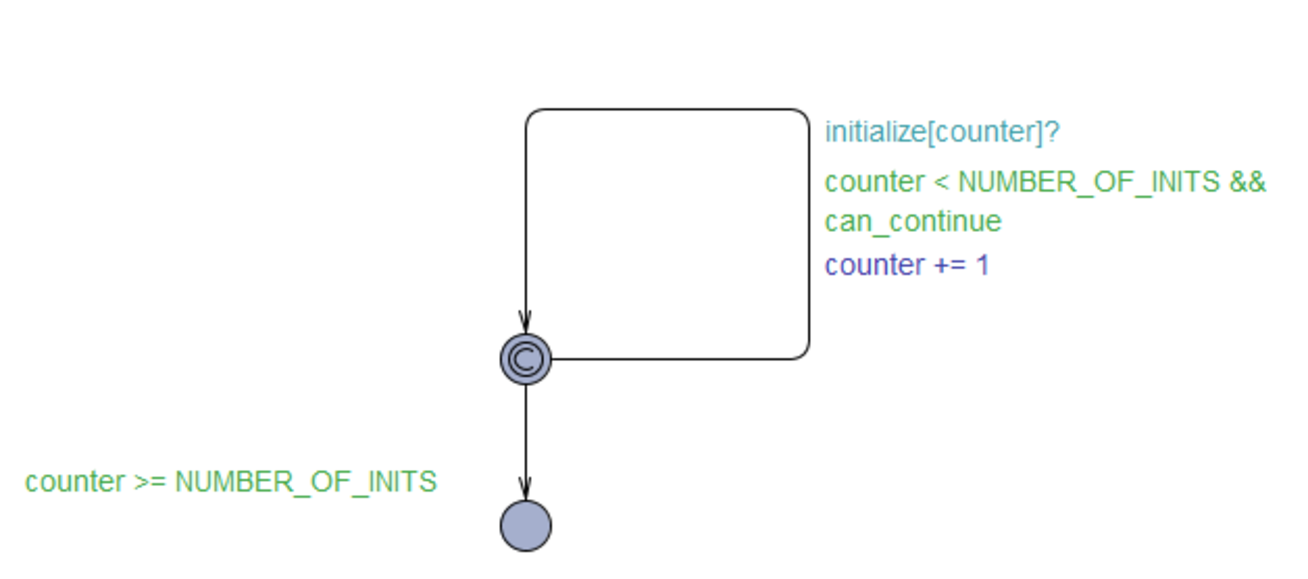
\includegraphics[width=\textwidth]{init.pdf}
\caption{The \textit{Initialzier} template}
\label{fig:initializer}
\end{figure}

